\documentclass[xcolor={dvipsnames}]{beamer}

\usepackage[T1]{fontenc}

\usepackage{amssymb}
\usepackage{stmaryrd}
\usepackage{amsfonts}
\usepackage{amsmath}
\usepackage{latexsym}
\usepackage{url}

\usepackage{listings}

\usepackage{mathtools}
\usepackage{calc}
\usepackage{lmodern}
\usepackage{changepage}
\usepackage{hyperref}
\usepackage{graphicx}

\usetheme{Madrid}

\setbeamertemplate{caption}{\raggedright\insertcaption\par}

\title[BeamBending]{Software Requirements Specification for ``Beam Bending''\newline{}\normalsize{}Examining a beam bending under load.}

\author[J. Balaci]{Jason Balaci}

\institute[McMaster U.]{McMaster University}
\date{Jan. $26^{\text{th}}$, 2023}

\AtBeginSection[]
{
  \begin{frame}
    \frametitle{Table of Contents}
    \tableofcontents[currentsection]
  \end{frame}
}

% For code highlighting
\usepackage[newfloat,outputdir=build]{minted}
\usemintedstyle{colorful}

% For loading images
\usepackage{graphicx}
\graphicspath{ {../assets/} }


% For fancy pictures
\usepackage{tikz}
\usetikzlibrary{shapes,arrows,cd}
\usetikzlibrary{babel} % Make sure quiver/tikz uses babel
\usetikzlibrary {arrows.meta,graphs,graphdrawing}
\usegdlibrary {layered}

\usepackage{todonotes}

\usepackage{svg}

\newcommand{\inlineHs}[1]{\mintinline{haskell}|#1|}
% Command based on: https://tex.stackexchange.com/questions/266811/define-a-new-command-with-parameters-inside-newcommand
\newcommand{\codeName}[1]{\expandafter\newcommand\csname #1\endcsname{\inlineHs{#1}}}

\codeName{CodeExpr}
\codeName{Expr}
\codeName{ModelExpr}

\begin{document}

%------------------------------------------------------------------------------
% TITLE
%------------------------------------------------------------------------------
\frame{\titlepage}

%------------------------------------------------------------------------------
% TABLE OF CONTENTS
%------------------------------------------------------------------------------

\begin{frame}
\frametitle{Table of Contents}
\tableofcontents
\end{frame}

%------------------------------------------------------------------------------
% OVERVIEW
%------------------------------------------------------------------------------
\section{Overview}

\begin{frame}
    \frametitle{Beam Bending}
  
    \begin{center}
        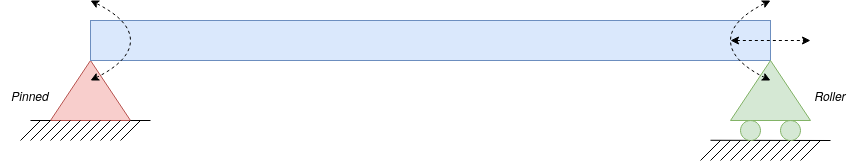
\includegraphics[width=0.9\textwidth]{temp/beam_bending_diagram.drawio.png}        
    \end{center}
\end{frame}

\begin{frame}
  \frametitle{Overview}

  \begin{enumerate}
    \item Background: Drasil
    \item 4 Research Areas:
      \begin{enumerate}
        \item Structuring theories
        \item Restricting mathematical expression terminology to appropriate
              contexts
        \item Well-typedness of mathematical expressions
        \item An extensible database for remembering everything
      \end{enumerate}
  \end{enumerate}

\end{frame}

%------------------------------------------------------------------------------
% BACKGROUND: DRASIL
%------------------------------------------------------------------------------
\section{Drasil}

\begin{frame}
  \frametitle{What is Drasil? How does it work?}
  \framesubtitle{\textquotedblleft{}Generate All The Things!\textquotedblright{}}

  \begin{columns}
    \begin{column}{0.45\textwidth}
      
\includegraphics[width=\textwidth]{drasil_logo.png}
    \end{column}
    \hfill
    \begin{column}{0.45\textwidth}
      \begin{enumerate}
        \item Software generation suite for ``well-understood'' domains
        \item De-duplicating and capturing knowledge across software artifacts
        \item Uses a Software Requirements Specification (SRS) template to
              decompose scientific problems and generate software
      \end{enumerate}
    \end{column}
  \end{columns}

\end{frame}

\begin{frame}
  \frametitle{Example}
  \framesubtitle{SRS to Code}

  \begin{columns}
    \begin{column}{0.45\textwidth}
      Using SRS components:
      \begin{enumerate}
        \item Symbols (inputs, outputs, and everything in-between)
        \item Problem description and goals
        \item Assumptions
        \item Abstract theories
        \item Concrete theories
        \item \(\ldots{}\)
      \end{enumerate}
    \end{column}
  \end{columns}

\end{frame}

%------------------------------------------------------------------------------
% CONCLUSION
%------------------------------------------------------------------------------
\section{Conclusion}

\begin{frame}
  \frametitle{Concluding Remarks \& Takeaways}

  To sum up, we\ldots{}
  \begin{enumerate}
    \item structured theories,
    \item restricted expressions by context,
    \item added type-checking to expressions,
    \item and prototyped an extensible chunk database structure.
  \end{enumerate}
\end{frame}

\end{document}
